\section{Results and Discussion}\label{sec:results}

Here, the results of the free energies of disappear the van der Waals interactions for 20 $n-alanines$ with n ranging from $1$ to $10$, in both configurations (helix and extended) are presented under the methods highlighted above.

\subsection{Energy Interaction Results}

First, the discrete transition between states A and B acopled with the $\lambda$-parameter, explained in Section \ref{subsec:TI} is presented in Figure \ref{fig:peptide_interactions}. 

\begin{figure}[h]
    \centering
    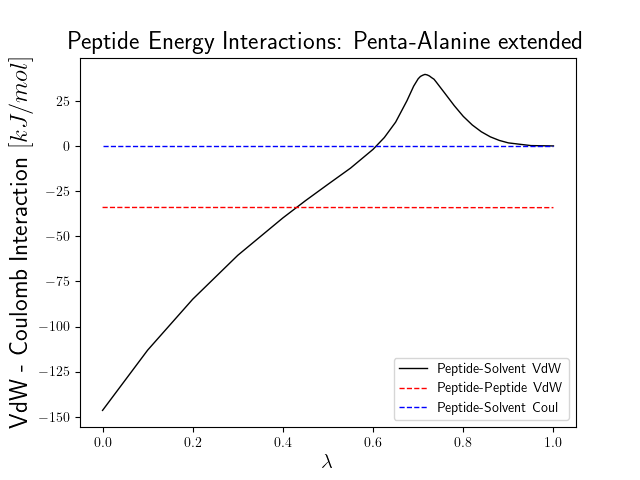
\includegraphics[scale=0.8] {Figures/Chapter_6/Interactions.png}
    \caption{Evolution of interactions between peptide and solvent while the transition of the $\lambda$ parameter.}
    \label{fig:peptide_interactions}
\end{figure}

The energy interactions between the peptide and the solvent is changed, using the soft core potential function (Equation \ref{eq:softcorepot}), from the initial value calculating with the force-fields parameters and the system configuration, to zero. Here, two important points must be notice: (1) the coulombic interactions is equal to zero during all the transition. This is because as it was said before, the atomic charges were manually set to zero (Section \ref{subsec:strucutre_prep}), and (2), the peptide-peptide interaction remains constant during the transition. This two factors, assures that the free energy change $\Delta G$ corresponds to the free energy required to turn-off the van der Waals interactions between the peptide and the solvent, i.e, the free energy of \textbf{generating the dry cavity on the solvent.} 

Figure \ref{fig:peptide_interactions} is a sample of the penta-alanine energy interactions in extended configuration, of all the 20 results. In addition, Figure \ref{fig:solvent_vdw} shows how the solvent van der Waals interactions evolves with itself during the transition of the $\lambda$-parameter.  
\begin{figure}[h]
    \centering
    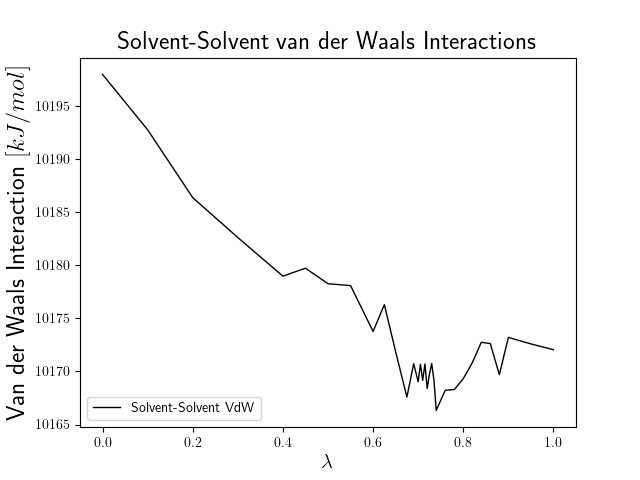
\includegraphics[scale=0.7]{Figures/Chapter_6/Solvent_vdw_Interactions.png}
    \caption{Evolution of van der Waals interactions between the solvent with itself while the transition of the $\lambda$ parameter.}
    \label{fig:solvent_vdw}
\end{figure}

Finally, the coulomb interaction between the solvent is presented in Figure \ref{fig:solvent_coul}. Notice that both interactions becomes more negative, i.e, more favorable during the transition because in the lack of interaction between molecules, or the presence of a dummy atom, allows the connection between more solvent molecules. We can think of this like the normal molecule is acting as a screen for the solvent molecules that are at the other side. in the process of tunr-off the peptide-solvent interactions, one can see how the solvent molecules that wasn't interacting with themselves, starts to contribute to the total value of these interactions. 
\begin{figure}[h]
    \centering
    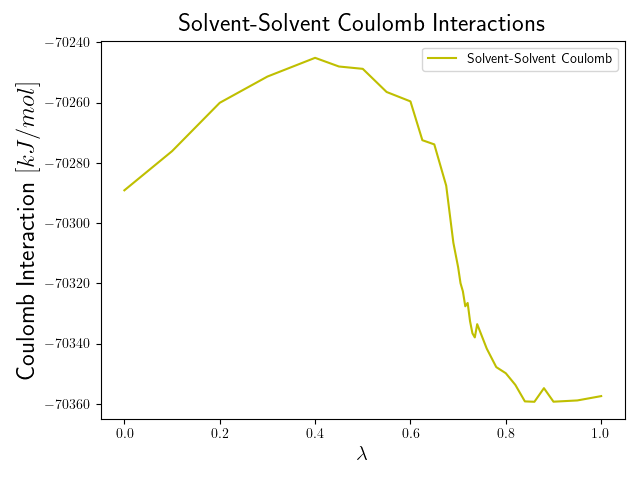
\includegraphics[scale=0.7]{Figures/Chapter_6/Solvent_coul_Interactions.png}
    \caption{Evolution of coulomb interactions between the solvent with itself while the transition of the $\lambda$ parameter.}
    \label{fig:solvent_coul}
\end{figure}

\subsection{Free energy Results}
Figure \ref{fig:TI_7ALA} illustrates the $\frac{\partial H}{\partial \lambda}$ values for each $\lambda$-points define in Section \ref{subsubsec:TIerror1}. This particular result correspond to the hepta-alanine ($ALA_7$) in helix configuration, and the total result of the free energy of solvation correspond to the integrate of all the points over the $\lambda$ space. 
\begin{figure}[h!]
    \centering
    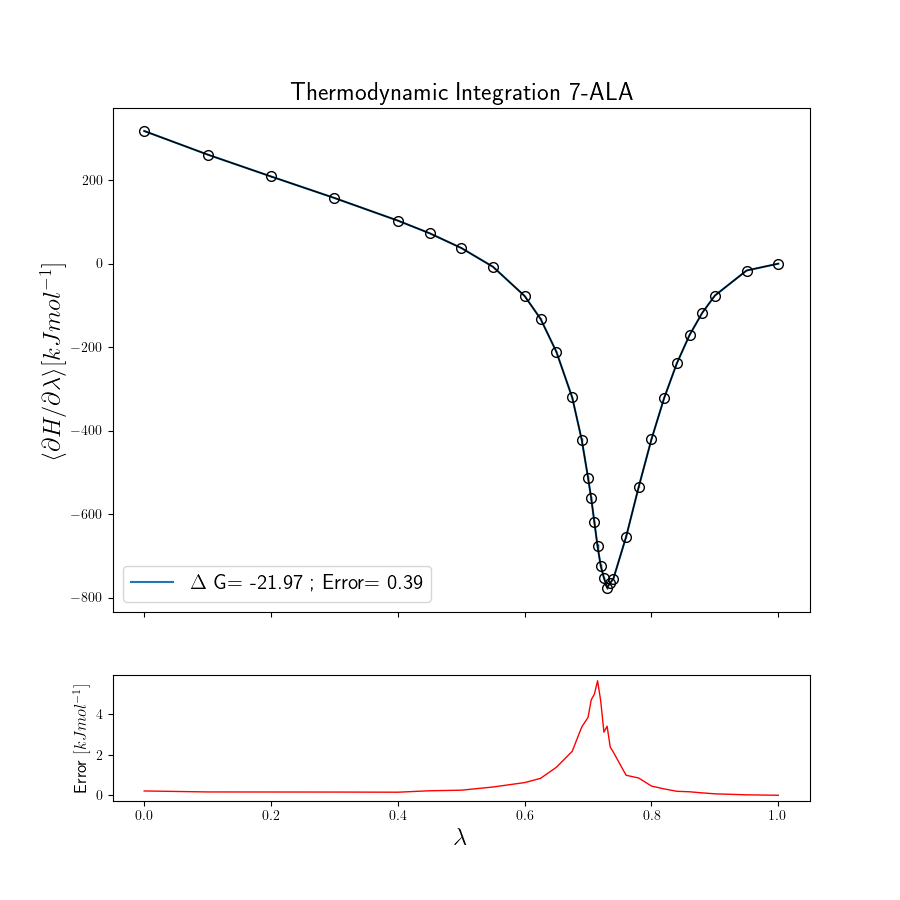
\includegraphics[scale=0.6]{Figures/Chapter_6/TI.png}
    \caption{TI curve for hepta-alanine in helix configuration.}
    \label{fig:TI_7ALA}
\end{figure}
This exercise was preform for every configuration and the results are presented as follows: Table \ref{table:DG_final} summarizes each numerical result for each configuration, both extended and helix, and Figure \ref{fig:DG_total} illustrates the free energies. All TI curves are attached to this work in the Appendix \ref{subsec:TI_curves}.


\begin{table}[th] %th for exact position.
    \centering
    \begin{tabular}{c|cc|cc}
    \toprule
    \multirow{2}{4em}{n-ALA}           &   \multicolumn{2}{c|}{\textbf{Helix}} & \multicolumn{2}{c}{\textbf{Extended}}\\

    &    $\Delta G_{cav}$ $[kJ/mol^{-1}]$ & Error $[kJ/mol^{-1}]$     &  $\Delta G_{cav}$ $[kJ/mol^{-1}]$    &    Error $[kJ/mol^{-1}]$  \\
    \midrule
    1         &   -6.350  &   0.153                  &   -7.752                 &   0.152\\
    2         &   -10.198  &   0.207                 &   -10.488                &   0.213\\
    3         &   -12.709  &   0.261                 &   -12.641                &   0.242\\
    4         &   -16.198  &   0.291                 &   -14.020                &   0.291\\
    5         &   -16.524  &   0.333                 &   -15.767                &   0.323\\
    6         &   -20.223  &   0.361                 &   -18.007                &   0.356\\
    7         &  -21.969  &   0.391                  &   -19.996                &   0.376\\
    8         &   -23.102  &   0.422                 &   -21.915                &   0.383\\
    9         &  -24.663  &   0.433                  &   -24.103                &   0.420\\
    10        &   -26.584  &   0.460                 &   -25.523                &   0.477\\
    \bottomrule
    \end{tabular}
    \caption{Summarize of the 20 free energies calculations with statistical error.}
    \label{table:DG_final}
\end{table}

\begin{figure}[h!]
    \centering
    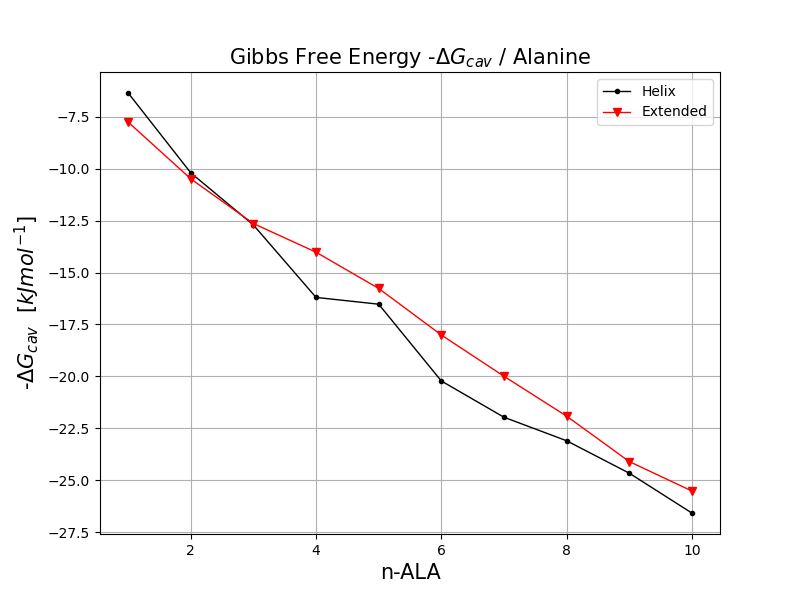
\includegraphics[scale=0.6]{Figures/Chapter_6/results_1.png}
    \caption{Solvation free energies of the extended and helix alanine peptides plotted as functions of the number (N) of residues in the peptide.}
    \label{fig:DG_total}
\end{figure}

As it it seen in Figure \ref{fig:DG_total}, a clear linear relationship between the size of the peptide that it is solvated, and the free energy required to generate the cavity it's seen. 

\subsubsection{Statistical Error}
As it is seen in Figure \ref{fig:TI_7ALA}, there are error values related to each $\lambda$-point. One can think that as a simulation is preform, there is no experimental measure to compare the results to estimate an error.
For this, GROMOS software calculate \textbf{averages} and \textbf{standard deviation} by blocks for to determine a \textit{statistical error} to each result. This is: all teh simulation samples are group in several blocks and for each block, the mean of the propertie of interest, is calculated. Then the mean of the mean of the blocks is reported and the standard deviation of this mean. This is because what we measure in general behaves like normal distributions, so the deviation does not tell us the error, but tells us other properties. But if we make blocks we can estimate as if we had made independent measurements, and from each one we have taken a single value (the average). Whit this, it's possible to report an error \cite{allen2017computer}. 

To estimate the precision of Equation \ref{eq:TI}, the following formula can be used for the standard deviation on the mean \cite{daura1996free}:
\begin{equation}
    \sigma\left ( \left \langle \frac{\partial H(\lambda )}{\partial \lambda } \right \rangle_{\lambda_n} \right ) = \left( \frac{S_{\lambda_n}}{N_{conf}} \right )^\frac{1}{2}\sigma\left (\frac{\partial H}{\partial \lambda}\right )
\end{equation}
where $N_{conf}$ denotes the number of configurations over which the ensemble average at $\lambda=\lambda_n$ is taken, and $\sigma\left (\frac{\partial H}{\partial \lambda}\right )$ is calculated as the square root of the variance over the ensemble.
\begin{equation}
    \sigma^2\left (\frac{\partial H}{\partial \lambda}\right )=\frac{1}{N_{conf}}\sum^{N_{conf}}_{t=1} \left[ \frac{\partial H}{\partial \lambda} - \left\langle\frac{\partial H}{\partial \lambda} \right \rangle_{\lambda_n,N_{conf}}\right ]^2
    \label{eq:statistical}
\end{equation}


To calculate the statistical inefficiency, $S_\lambda_n$, the total simulation time at $\lambda=\lambda_n$ is divided into $M$ blocks of length $b$, and $N_b$ configurations are taken from each block such that $M\cdot N_b=N_{conf}$ \cite{allen2017computer}. The variance of the mean is then calculated for each possible block length $b$ as: 
\begin{equation}
     \sigma^2\left ( \left \langle \frac{\partial H(\lambda )}{\partial \lambda } \right \rangle_{\lambda_n,b} \right ) = \frac{1}{M}\sum^M_{m=1}\left[ \left\langle\frac{\partial H}{\partial \lambda}\right\rangle_{\lambda_n,N_b,m}- \left\langle\frac{\partial H}{\partial \lambda} \right \rangle_{\lambda_n,N_{conf}}\right ]^2
\end{equation}
where $\left\rangle ... \right\rangle_{\lambda_n,N_b,m}$ denotes the ensemble average at $\lambda = \lambda_n$ over $N_b$ configurations of the $m-th$ block. $S_\lambda_n$ is then calculated as: 

\begin{equation}
    S_\lambda_n=\lim_{N_b\rightarrow \infty }\frac{N_b \sigma^2\left ( \left \langle \frac{\partial H(\lambda )}{\partial \lambda } \right \rangle_{\lambda_n,b} \right )}{ \sigma^2\left (\frac{\partial H}{\partial \lambda}\right )}
\end{equation}
\par
It is the limiting ratio of the observed variance of an average to the limit expected on the
assumption of uncorrelated Gaussian statistics. Having estimated $S_\lambda_n$, we can write Equation \ref{eq:statistical}. This statistical error is presented in Table \ref{table:DG_final} and in the bottom graph in Figure \ref{fig:TI_7ALA}. This error is corrected by extending the simulation time for the TI because it generates more configuration to sample. This is the main reason why in Section \ref{subsec:MDS} the simulation time for the TI was determined at $15 [ns]$. 

\subsection{Comparison Between Models}\label{subsec:comparison}
For the standard SASA model, described in Equation \ref{eq:G_solv}, $\Delta G_{cav}$ is computed with $\gamma = 2.51 [kJ/mol/nm^2]$ or $0.06 [kcal/mol/\AA^2]$ and $b = -12.55 [kJ/mol]$ or $-3 [kcal/mol]$. For the propose implicit solvent model, the following constants were used according to Equation \ref{eq:CC_implicit}: $\Phi_{static} = 10.7 [kcal/mol/e]$, $\epsilon_{shell} = 7.75$, and $\rho_{shell}=1.8\rho_w$, with $\rho_w=0.0336 \AA^{-3}$ the bulk water density. All this parameters were selected to calibrate the model after compared the results with the Mobley's explicit-solvent free energy perturtabtion (FEP) calculations \cite{mobley2009small}. Figures \ref{fig:helix_comparison} and \ref{fig:ext_comparison} shows these results. 

\begin{figure}[h]
    \centering
    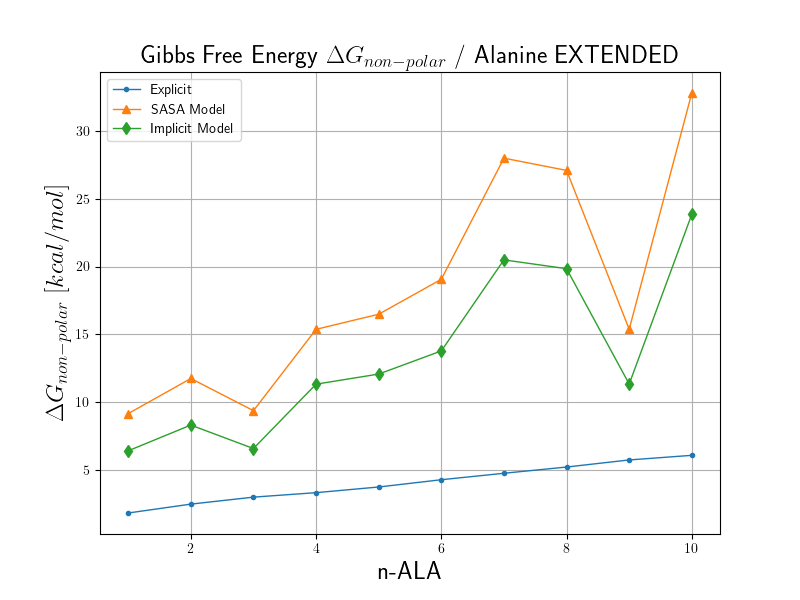
\includegraphics[scale=0.65]{Figures/Chapter_6/comparison_extended.png}
    \caption{Gibbs free energy results from the three models described in this work for extended configuration, per alanine peptide.}
    \label{fig:ext_comparison}
\end{figure}

\begin{figure}[h]
    \centering
    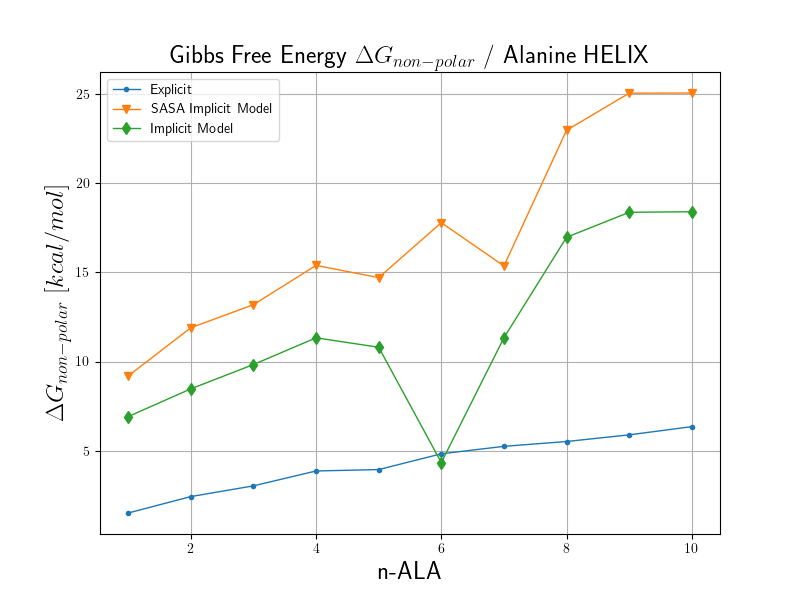
\includegraphics[scale=0.65]{Figures/Chapter_6/comparison_helix.png}
    \caption{Gibbs free energy results from the three models described in this work for helix configuration, per alanine peptide.}
    \label{fig:helix_comparison}
\end{figure}


The use of parametrizations, like the constants described in Section \ref{subsec:comparison}, or the force-field use for the simulations, implies an intrinsic source of uncertainty specially because the lac of empirical measurements related to the free energy calculations. 

As it's seen in Equation \ref{eq:G_solv} and \ref{eq:CC_implicit}, both models depends strongly on the SASA parameter. The standard SASA model can be interpreted as a linear correlation dependent on the SASA factor, and the Implicit solvent model, uses this surface to integrate the potential on it (Eq. \ref{eq:int_shell}). Depending on the method used to generate the SASA factor, both models can carry inaccuracies on the calculations. Figure \ref{fig:SASA_comparison} present the results of tho methods to obtain the SASA factor, one with GROMOS program \texttt{sasa} and the other generated with \texttt{msms} and used in the implicit model.

\begin{figure}[h]
    \centering
    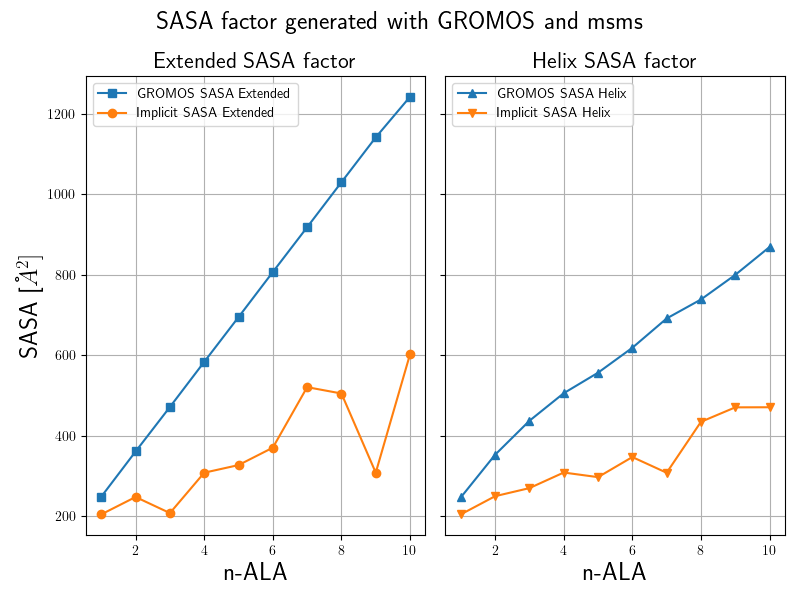
\includegraphics[scale=0.6]{Figures/Chapter_6/SASA_factor.png}
    \caption{Differences between SASA factor generated with \texttt{GROMOS} software and \texttt{msms} program.}
    \label{fig:SASA_comparison}
\end{figure}

The calculation with implicit and standard sasa model (Figure \ref{fig:helix_comparison} and \ref{fig:ext_comparison}), shows ``anomalies" in the free energy values in ($ALA_{9}-extended$) and 
($ALA_{6}-helix, ALA_{7}-helix$). This is correlated with the same behavior in SASA factors showed in Figure \ref{fig:SASA_comparison} which generates the free energy results. To correct this, the method to generate the mesh around the peptide coordinates must be fixed, for example, using a probe with higher molecule radius. 

To measure the accuracy of the prediction for $\Delta G_{np}$ of both models, Pearson coefficient $\rho_p$, root mean square of the difference (RMSD) and the correlation coefficient $R^2$ are used and presented in Table \ref{table:measures_1}. 

\begin{table}[th] %th for exact position.
    \centering
    \begin{tabular}{c|ccc|ccc|c}
    \toprule
    \multirow{2}{4em}{Model}           &   \multicolumn{3}{c|}{\textbf{Helix}} & \multicolumn{3}{c}{\textbf{Extended}}&\textbf{Total}\\

    &   $R^2$ & RMSD   &   $\rho_p $ &  $R^2$ & RMSD   &   $\rho_p $ & \textbf{RMSD}\\
    \midrule
    SASA Model & 0.853 & 22.339 & -0.949 & 0.651 & 24.216 & -0.807 & 23.296\\
    Implicit Model & 0.503 & 16.939 & -0.709 & 0.661 & 18.791 & -0.813 & 17.889\\      
    \bottomrule
    \end{tabular}
    \caption{Comparison of $\Delta G_{np}$ between standard SASA model and the Implicit model proposed.}
    \label{table:measures_1}
\end{table}     

With the parameters described at the beginning of this section, the implicit solvent model presents an improvement of 22.53 \% in predicting the free energy of solvation $\Delta G_{cav}$ over the standard SASA model. 

\subsubsection{Adjust Models constants}

To improve the accuracy of both implicit models, one can adjust the constants to fit the explicit MD curve and improve the overall forecast result. Taking this into account, modifications to both models were made: First, related to the standard SASA model, we propouse the values of $\gamma = 0.025$ and $b = -4.1$ in contrast to the values presented above \cite{cooper2020simple}. Second, we propose a value of $\epsilon_{shell}=3.1$ in contrast to the value reported in \cite{cooper2020simple} of $\epsilon_{shell}=7.75$ as a fitting parameter. The result of this consideration are presented in Figure \ref{fig:new_cc}. Table \ref{table:measures_2} summarizes the results with the new parametrizatrion. 

\begin{figure}[h]
    \centering
    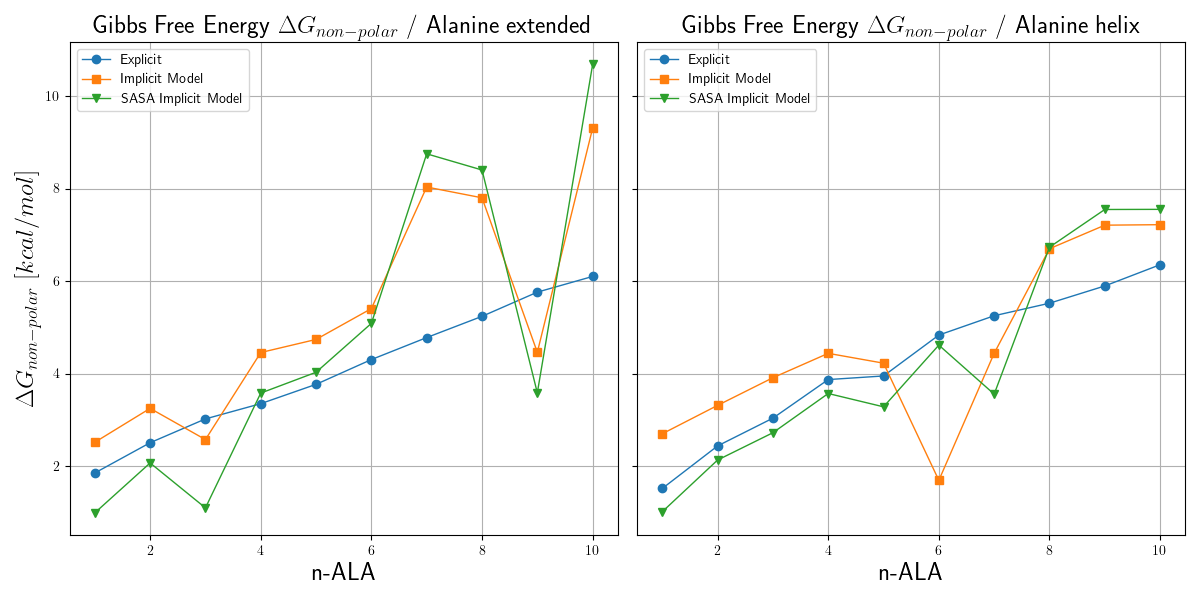
\includegraphics[scale=0.52]{Figures/Chapter_6/New_CC.png}
    \caption{Results after adjustment of parameters $\gamma = 0.025$, $b = -4.1$ for SASA standard model, and $\epsilon_{shell}=3.1$ for the implicit model presented in this work.}
    \label{fig:new_cc}
\end{figure}

\begin{table}[th] %th for exact position.
    \centering
    \begin{tabular}{c|ccc|ccc|c}
    \toprule
    \multirow{2}{4em}{Model}           &   \multicolumn{3}{c|}{\textbf{Helix}} & \multicolumn{3}{c}{\textbf{Extended}}&\textbf{Total}\\

    &   $R^2$ & RMSD   &   $\rho_p $ &  $R^2$ & RMSD   &   $\rho_p $ & \textbf{RMSD}\\
    \midrule
    SASA Model & 0.852 & 9.269 & -0.949 & 0.653 & 9.905 & -0.808 & 9.592\\
    Implicit Model & 0.501 & 9.364 & -0.708 & 0.662 & 9.935 & -0.814 & 9.654\\      
    \bottomrule
    \end{tabular}
    \caption{Comparison of $\Delta G_{np}$ between standard SASA model and the Implicit model with the re-parametrization.}
    \label{table:measures_2}
\end{table}     

\subsection{Conclusions}

In this work, we studied the contribution of van der Waals interactions in the solvation free energy using the Molecular Dynamics (MD) method. This computer simulation methodology allows us to analyze the physical movements of atoms and molecules which are interacting between them for a fixed period of time and used to extract macro-thermodynamic properties like, in this case, free energies. 
The solvation free energy is the energy cost of the process of reorganizing solvent and solute molecules into solvation systems. The solvation process describes the interaction between the solute and solvent molecules and it is govern by electrostatic and van der Waals interactions. In this case, we focus on the free energy which is calculated by the second component. 
To analyze how the property changes with the size of the molecule, 20 alanine-peptide structures were prepared ranging from 1 to 10, and in helix and extended configuration. Finally, free energy results were calculated using the Thermodynamic Integration (TI) method during a MD run. 

From all the 20 TI, it was clear the linear relation between the volume (size) of the alanine peptides, represented in Figure \ref{fig:DG_total}, which is an expected result. If one want to solvate a bigger molecule, higger free energies will result from these solvation processes. In the other hand, as we add identical residues to the next alanine-peptide, from $ALA_1$ to $ALA_2$, from $ALA_2$ to $ALA_3$ and so on, we expect a linear constant characteristic from the alanine peptide. 

We also analyze two implicit methods to estimate this free energy change. One standard method that relates the Solvent-Accessible Surface Area (SASA) with some fitting constants ($\gamma = 0.06 [kcal/mol/\AA^2]$ and $b = -3 [kcal/mol]$) that have shown high accurate results, and a new method that relies in a clearer physical meaning and formulation which uses a capacitor model to emulate the interaction distribution around the solvated peptide. 

To compare the accuracy of the implcit models, the calculations generated with the explicit-MD simulation was used as the ``real/observed" result, and contrast them with the implicit results. It was found the new method for calculating the solvation free energy, and with the parameters described in this work, improves the estimation of the thermodinamic property by \textbf{22.53\%} acording to RMSD parameter. 

It is also proposed a re-parametrization of the fitting constants according to the results presented in this work of $\gamma = 0.025$ and $b = -4.1$ in the case of the standard SASA model, and $\epsilon_{shell}=3.1$ for the propoused implicit solvent model. 




 